\chapter{Result From Flight Data}\label{ch:FlightResult}

This chapter discussed the result of applying the proposed algorithm
on realistic aerial video and navigation data. Firstly, a piece of
video of 400 frames were processed by the CC\_EKF\_SLAM algorithm. The
convergence, accuracy and consistency of the result were analyzed
against ground truth, and described in section
\ref{sec:flight-converge}-\ref{sec:flight-consistency}. While
analyzing pure natural scene video where no man-made object can be
seen, it was found that landmarks correspondence between the
estimated and ground truth was difficult due to the
similarity in apperance of the landmark. Therefore, an another video
where landmarks can be manually and distinctively matched was
processed, and result was summarized in section \ref{sec:flight-manual}.

\section{Convergence}\label{sec:flight-converge}
When a landmark was added to the filter, the landmark initialization
point were initialized to the zero which is the origin of the camera
centric coordinate. $\phi$ and $\theta$ were calculated directly from
the feature position on image plane, had relatively high accuracy, and
should stay relatively constant. The only parameter that experienced
a converging process was the inverse depth $\rho$, which were
initialized to 0.1 for all landmarks.

Figure \ref{fltfig:1} shows the $1/\rho$ plot for the entire 400
frames. Landmark ID was shown on the right side of the plot for the
landmarks that were not converging. The depth estimates went through
rapid changes for several frames after initialization. Within
approximate 20 frames, most inverse depth estimates settled to stable
values. Sharp spike in the middle of the tracking is due to new
landmarks added into the filter. The estimated landmarks distances
ranged from 400 meters to about 1200 meters, confirming the
algorithm's capability for estimating landmarks at great distance. On
the other hands, some landmarks took a long time to settle, while some
other never settled and drift away as tracking continued, such as
landmark 32, 13, and 53. 
% An outlier filter should be in place to get rid of the poor features
% (future work).

\begin{figure}[h]
\centering
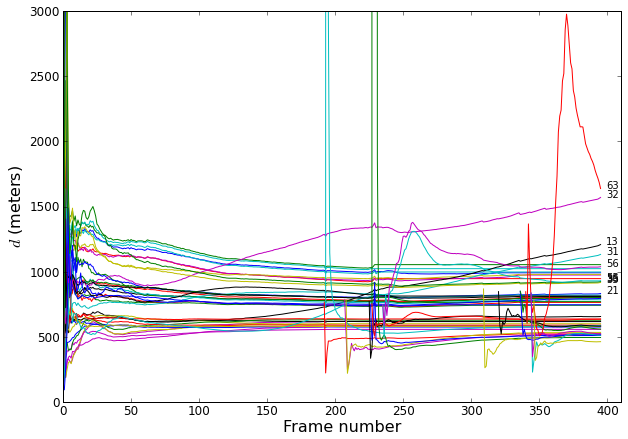
\includegraphics[width=12cm, keepaspectratio=true]{./Figures/fltfig/cut1/Figure10.png}
\caption{Inverse Depth Convergence}
\label{fltfig:1}
\end{figure}

The non-converging landmarks were those located at the edge of a hill
where objects with big difference in distance meet in the image. As an
example, visual pattern of landmark 13 at frame 50, 100, 150, 200,
250, 300, 350 and 398 were shown in figure \ref{fltfig:1_1}. It showed
that the initial visual pattern for landmark 13 was detected at the
edge of a hill top. As frame number advanced, the view the camera
became different. The pattern comparison in tracking algorithm
normally allows for a small error at each iteration to tolerate the
slight view change of the camera. This error accumulated slowly and
eventually caused the tracked target to become a pattern located at a
different location, which explained the slow drift in depth estimate.
To increase the reliability of the estimates, it is necessary to add
procedure into the algorithm to detect and handle such behavior.

\begin{figure}[h]
\centering
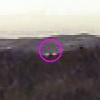
\includegraphics[width=3cm,
keepaspectratio=true]{./Figures/fltfig/cut1/features/uav2_cut1_050_fID13.jpg}
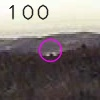
\includegraphics[width=3cm,
keepaspectratio=true]{./Figures/fltfig/cut1/features/uav2_cut1_100_fID13.jpg}
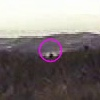
\includegraphics[width=3cm,
keepaspectratio=true]{./Figures/fltfig/cut1/features/uav2_cut1_150_fID13.jpg}
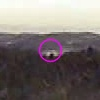
\includegraphics[width=3cm,
keepaspectratio=true]{./Figures/fltfig/cut1/features/uav2_cut1_200_fID13.jpg}
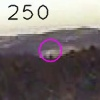
\includegraphics[width=3cm,
keepaspectratio=true]{./Figures/fltfig/cut1/features/uav2_cut1_250_fID13.jpg}
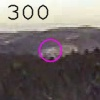
\includegraphics[width=3cm,
keepaspectratio=true]{./Figures/fltfig/cut1/features/uav2_cut1_300_fID13.jpg}
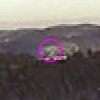
\includegraphics[width=3cm,
keepaspectratio=true]{./Figures/fltfig/cut1/features/uav2_cut1_350_fID13.jpg}
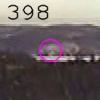
\includegraphics[width=3cm,
keepaspectratio=true]{./Figures/fltfig/cut1/features/uav2_cut1_398_fID13.jpg}
\caption{Landmark 13 at frame 50, 100, 150, 200, 250, 300, 350, and 398}
\label{fltfig:1_1}
\end{figure}

When landmarks were initialized, the initialization coordinate $[x_i,
y_i, z_i]$, and the deviation-elevation angle pair $[\varphi, \theta]$
did not go through a slow converging stage. Ideally, the parameters
should stay at a relatively fixed value. As these parameters were used
with the inverse depth to calculate landmark coordinates on image
plane and received every iteration, their values were affected by the
inverse depth, and varied at each iteration. The plots in figure
\ref{fltfig:2} showed the variation of these parameters over the
entire processed frames.

First column of the plots showed landmark initialization coordinates
with the initial value subtracted. All landmarks that were initialized
at $1^{st}$ image frame had stable value with little variation.
Landmarks that were added at later image frames showed significant
drift from their initial value. This is a direct result of the filter
correction process. When a new landmark were added to the filter, it
had not established correlation with all the other landmarks and the
world frame parameters, which caused its correction on initialization
point slightly different than all the existing features and the world
frame position. As a future improvement, it is reasonable for the
newly added landmark to inherent the cross-correlation on the
initialization coordinates from a landmark close to it. elements.

Second and third columns showed elevation $\varphi$ and deviation
$\theta$ with their initial value or mean value subtracted.
For all landmarks, whether initialized at first image frame, or later
frames, these angle estimates all diverged slightly from the initial
values. This is not surprising since the initial depths of the
landmarks were unknown. To compensate for the incorrect depth, filter
must change $\varphi$ and $\theta$ estimates slightly to arrive at a
predicted measurements that agreed with the actual measurements.
Secondly, the SUAS rotation motion contributes to the variation
pattern of $\varphi$ and $\theta$ estimates.
\colorbox{yellow}{$\varphi$ is highly correlated with the Z rotation,
  and $\theta$ is correlated to the X rotation.(Verification
  required).} This behavior suggested that the algorithm might be
highly sensitive to aircraft rotational motion.
% doesn't make sense. By definition, X rotation should have bigger
% impact on varphi, Z rotation has bigger impact on theta

\begin{figure}[h]
\centering
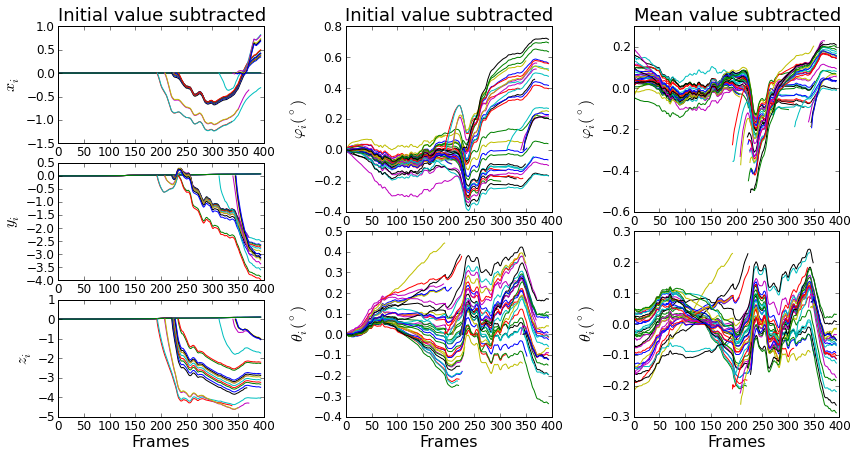
\includegraphics[width=14cm, keepaspectratio=true]
{./Figures/fltfig/cut1/Figure20.png}
\caption{Landmarks parameters tracking}
\label{fltfig:2}
\end{figure}
% THIS WAS THE OLD TEXT, MAY NOT BE TRUE. On the other hand, features
% mapping is not affected too much by the error in localization.
% Because their parameters are transformed in each iteration to the
% new camera frame using the estimated SUAS motion which carries the
% error. As long as their parameters are updated together with the
% estimated motion on that iteration, and transformed back to the
% world frame using the same estimated motion, the final result of
% features location in world frame is unaffected by the error in the
% SUAS localization. However, for feature removed from the filter,
% their parameters are no longer updated, therefore revealing the
% error in SUAS localization.
\FloatBarrier

\section{Accuracy}\label{sec:flight-accuracy}
\subsection{SUAS Localization}

Ground truth for SUAS position and orientation came from the GPS, and
magnetometer. The GPS positioning can generally achieve 7.8 meters in
accuracy \cite{_gps_????}. For orientation, accuracy on the GS-111m
datasheet specified $0.1^{\circ}$ for roll and pitch, and
$0.5^{\circ}$ for heading. Figure \ref{fltfig:6} shows the estimated
SUAS position and orientation, ground truth data, and the error. From
the comparison, X position error reached a maximum of 4.8 meters,
while error on Y and Z are bigger, reaching 60 meters and 28 meters
respectively. The position on Y axis were clearly diverging from the
ground truth by the end of 400 frames. For orientation, the estimated
value agreed with the ground truth pattern, with maximum error within
0.02 rad or $1.15^{\circ}$. There was no clear sign of diverging
within the 400 frames processed. Another character that can be
observed is the correlation between the position errors and the
aircraft orientation. Error on Y position was correlated to
orientation on Z axis; error on Z position was correlated to
orientation change on Y axis. Clearly, aircraft rotational motion
plays a crucial part in the accuracy of the estimates.

\begin{figure}[h]
\centering
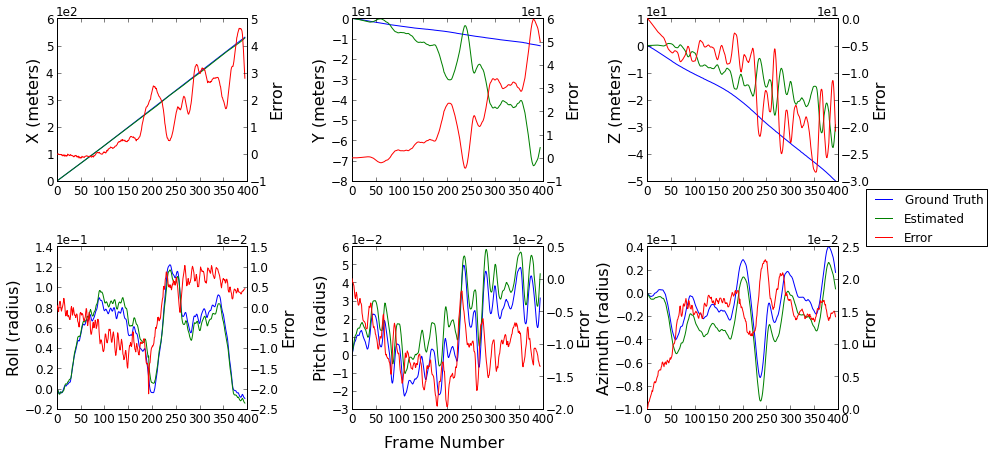
\includegraphics[width=15.5cm, keepaspectratio=true]
{./Figures/fltfig/cut1/Figure30.png}
\caption{SUAS position and orientation}
\label{fltfig:6}
\end{figure}
\FloatBarrier
\subsection{Landmarks Mapping}\label{sec:accuracy_features}

The ground truth data came from digital terrain map (DEM) were
downloaded from CGIAR-CSI website \cite{_cgiar-csi_????}. Data
correspondence between the DEM and the estimated landmarks is
non-trivial for natural scene where it lacks distinguishable visual
features such as building corners or other man-made objects. The
converging plots figure \ref{fltfig:2} showed that landmark parameters
do experience drift as filter tracked landmarks in flight. The best
time for making data correspondence with DEM is when landmarks were
first initialized. The landmark initialization position $[x_i, y_i,
z_i]$ were zeros when landmarks were initialied. $[\varphi,
\theta]$ were calculated from landmark coordinates in image, and did
not carry any error contributed by the $\rho$ or optical flow
algorithm result. Therefore, the following procedure were used the find
the corresponding ground truth location for every estimated landmark.

\begin{enumerate}
  \item The frame number at which landmark was initialized was
  identified. Ground truth position of the SUAS at that frame was
  recorded.
  \item Create a reference frame aligned with the UTM frame on DEM
  using the ground truth SUAS position.
  \item Convert the landmark parameters $\theta$ and $\varphi$
  angle at initialization from camera frame to UTM frame. 
  \item Create a vertical plane using $\theta$ to slice the DEM to
  form a 1D elevation plot. A example result was shown in figure
  \ref{fltfig:7} blue line.
  \item Create a line using $\varphi$ to intersect the 1D elevation plot
  (Figure \ref{fltfig:7} green line). 
  \item The $1^{st}$ intersection was used as ground truth landmark
  location.
\end{enumerate}

\begin{figure}[h]
\centering
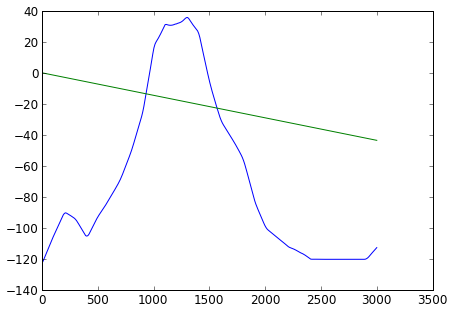
\includegraphics[width=10cm, keepaspectratio=true]
{./Figures/fltfig/cut1/intersect0_0.png}
\caption{Finding ground truth feature position on DEM}
\label{fltfig:7}
\end{figure}

The convergence of landmark position error was plotted in figure
\ref{fltfig:8}. X component (along which axis the SUAS was traveling)
converged to zero in general with error ranging from 2.8 meters to 120
meters. Y component showed a clear offset for landmarks not initialized
at first frame. This behavior is similar to what's seen in the
error analysis \ref{sec:featureMotion} where offset in landmarks
position estimates were caused by drift in SUAS localization
estimation. Offset on Z component was much less obvious.

\begin{figure}[h]
\centering
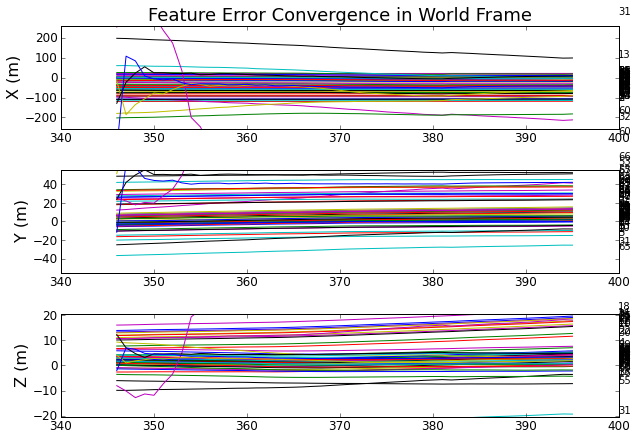
\includegraphics[width=10cm, keepaspectratio=true]
{./Figures/fltfig/cut1/Figure50.png}
\caption{Landmarks position error convergence in world frame}
\label{fltfig:8}
\end{figure}

Landmark IDs were assigned to landmarks sequencially when landmarks
were initialized into the filter. Plotting the estimated and ground
truth landmarks position against landmark ID revealed more detail on
the errors. Figure \ref{fltfig:9} plotted the estimated and ground
truth landmark positions on the left, and error on the right. On X and
Z component, the biggest error occurred on landmark number 65 which
was initialized fairly late in the sequence, and may not have
converged properly. Other landmarks that carry big errors, such as
landmark 13, 31, and 32, all located on hill top, which appeared as
line feature in image (Figure \ref{fltfig:line_features}). As visual
tracking drift discussed earlier applied to all these line features,
distance estimates accuracy on these landmarks were affected. On Y
axis, the plots showed landmark ID higher than 40 carried an offset
error. All landmarks with ID higher than 40 were initialized after
frame 180, at which point the SUAS has travelled away from the world
frame origin for at least 200 meters. The average error increased as
landmark ID got bigger, which indicated that the further the landmark
initialization point was from the world frame origin, the bigger the
offset error became. A more systematic analysis were done to find the
source of these offset errors, and the result were presented in
chapter \ref{ch:simulation}.

\begin{figure}[h]
\centering
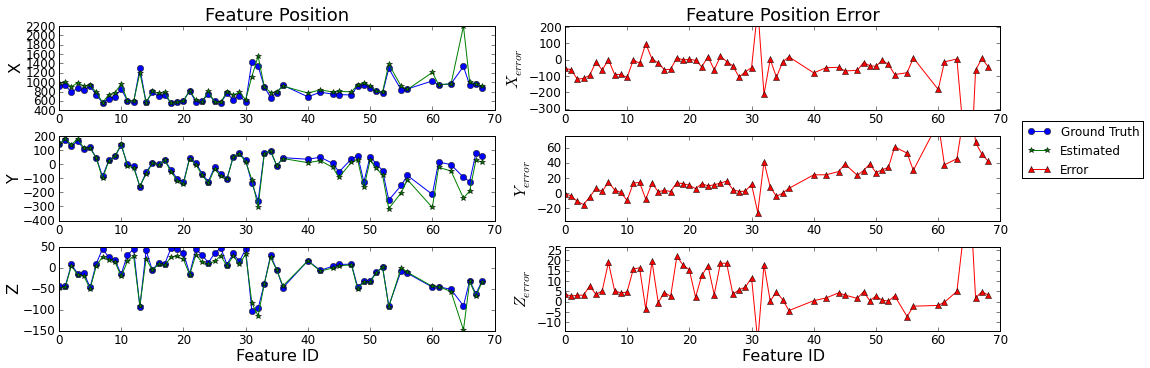
\includegraphics[width=16cm, keepaspectratio=true]
{./Figures/fltfig/cut1/Figure60.png}
\caption{Landmark position error plotted against initialization sequence. }
\label{fltfig:9}
\end{figure}

\begin{figure}[h]
\centering
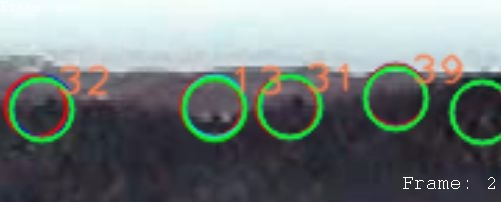
\includegraphics[width=7cm, keepaspectratio=true]
{./Figures/fltfig/landmark_13_31_32.jpg}
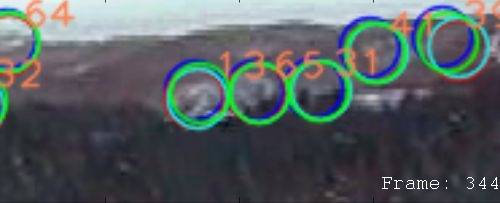
\includegraphics[width=7cm, keepaspectratio=true]
{./Figures/fltfig/landmark_13_65_32.jpg}
\caption{Landmarks on hill top carries bigger error during tracking.}
\label{fltfig:line_features}
\end{figure}

Using the estimated landmark position, a terrain map can be generated.
Figure \ref{fltfig:10} showed the terrain map generated from the
landmark position analyzed above. On the right, the ground truth DEM was
also shown for comparison. 

\begin{figure}[h]
\centering
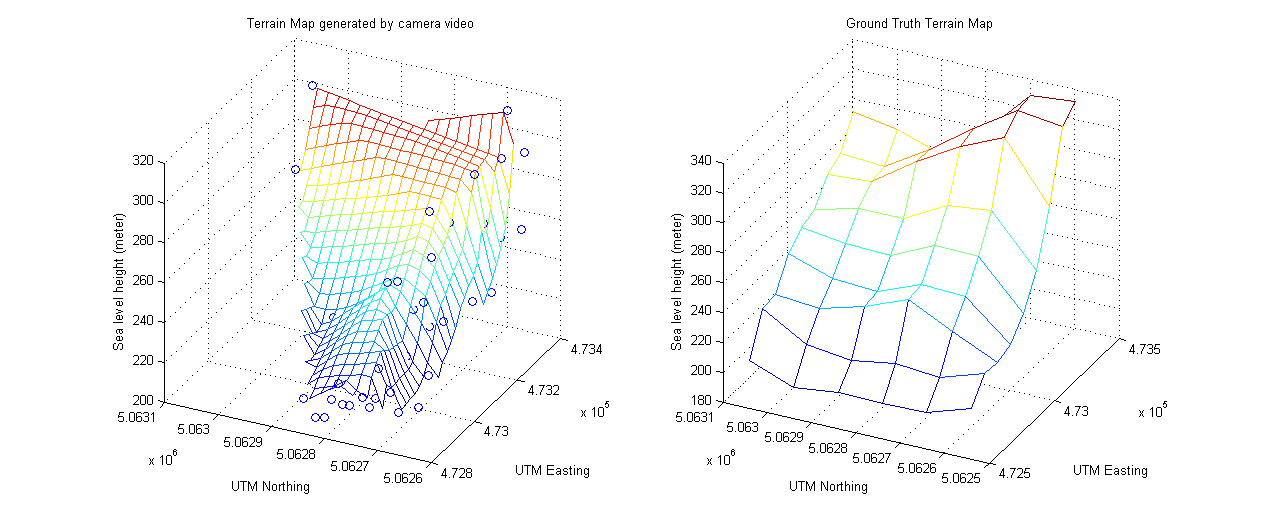
\includegraphics[width=14cm, keepaspectratio=true]
{./Figures/fltfig/cut1/terrain/terrain_map_cmp.png}
\caption{Terrain map. Left: estimated, right: ground truth }
\label{fltfig:10}
\end{figure}
\FloatBarrier

\section{Consistency Analysis}\label{sec:flight-consistency}
Researches on EKF SLAM properties indicated that 
\begin{enumerate}
  \item A EKF system becomes inconsistent when variance of a state
  vector element becomes too small and forbids an effective update,
  \item Uncertainty of the world frame should increase as the
  camera frame moves away from it.
\end{enumerate}

To examine the consistency of the CC\_EKF\_SLAM algorithm, the
variance of world frame parameters and camera motions were plotted in
\ref{fltfig:120}, and variance of landmarks parameters were plotted in
figure \ref{fltfig:3}. The variance of world frame position increased
with iterations at the beginning. After frame 100, $\sigma^2_{O_Y}$
and $\sigma^2_{O_Z}$ converged to a relatively stable value. This is
likely due to the small and slow variation on the Y and Z translation
of the SUAS. On the other hand, camera rotation and world frame
orientation variance had similar pattern and amplitude. The X
component decreased with iterations. Y and Z components fluctuated
around a fixed value and remained below 1.5e-5$^\circ$. Although world
frame orientation variance remained fixed at prediction, camera
rotation variances had 1$^\circ$ of noise added at the prediction step (as
indicated by the GS-111m specification \cite{_athena_????}). The
update process reduced the noise of camera rotation significantly and
resulted in a variance estimates much lower than the specification.
Affected by the camera rotation variance, landmarks parameters
$\varphi$ and $\theta$ also had very small variance.

% does increasing measurement variance increases parameter variance?
% answer: NO 

\begin{figure}[h]
\centering
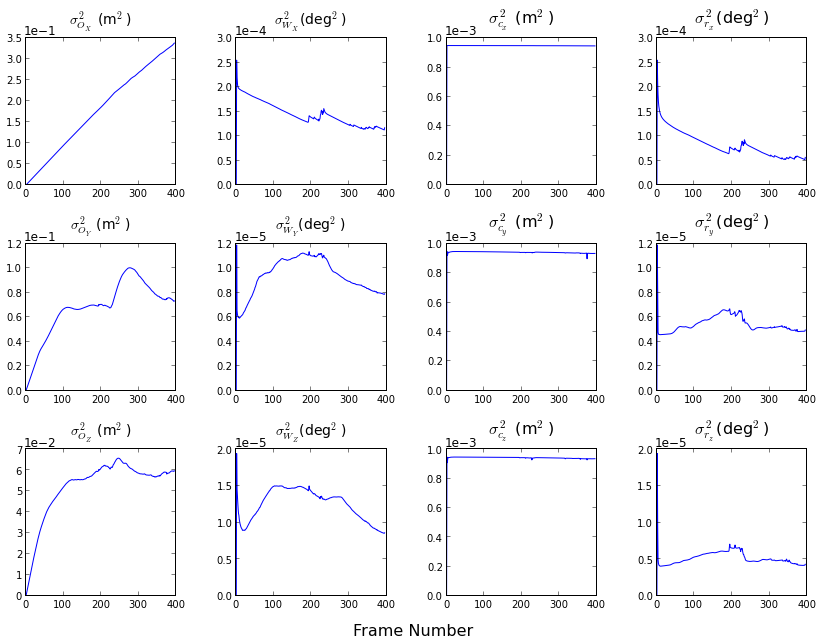
\includegraphics[width=14cm, keepaspectratio=true]
{./Figures/fltfig/cut1/Figure120.png}
\caption{Variance of world frame parameters and camera motion}
\label{fltfig:120}
\end{figure}


\begin{figure}[h]
\centering
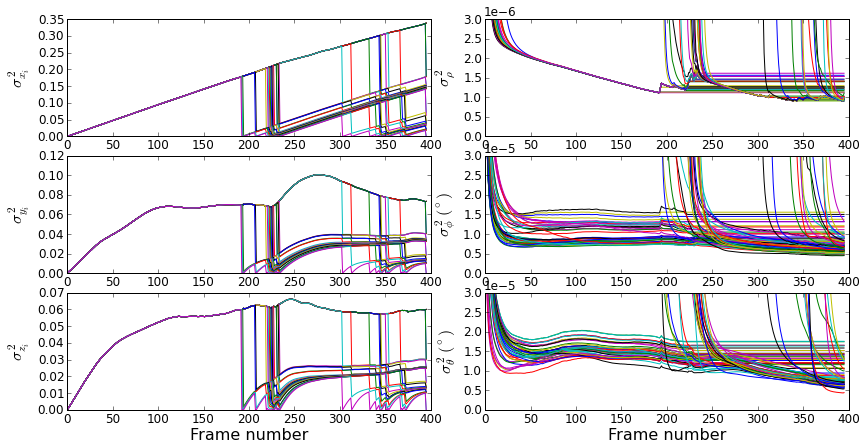
\includegraphics[width=14cm, keepaspectratio=true]
{./Figures/fltfig/cut1/Figure40.png}
\caption{Variance of landmarks parameters}
\label{fltfig:3}
\end{figure}
\FloatBarrier

% consider deleting first and second point in the paragraph. Only the
% third point leads to explaination of error.
To see the effect of small variance on EKF's update process, correction
amount applied to the predicted state vector were plotted in figure
\ref{fltfig:4}. It can be observed that in general the correction
amount agreed with the variance that bigger variance resulted in more
correction, except for the world frame position and camera translation
on Y and Z axis. These parameters received more correction as tracking
progress despite their variance stabilized or even decreased.
Secondly, there was a strong correlation between the landmark
initialization position, the world frame position, and camera
translation estimates. World frame position and landmark
initialization were inversly correlated to the camera translation on Y
and Z axis. Thirdly, the camera parameter corrections showed an
obvious trend only on Y and Z motion. The correction amounts on camera
translation on Y and Z axis were increasing with time. Due to these
relationship, the main contributor for drift in SUAS position and
offset in landmark mapping should be the camera translation correction
on Y and Z axis. On the other hand, the big correction on these
parameters could be caused by the small variance in the camera
rotation variance. If not enough correction can be made into the
camera rotation and $\varphi$ and $\theta$ angles, the algorithm must
compensate that by making more adjustment in the camera translation on Y
and Z axis. This issue requires further investigation, and will be analyzed
in future work.

\begin{figure}[h]
\centering
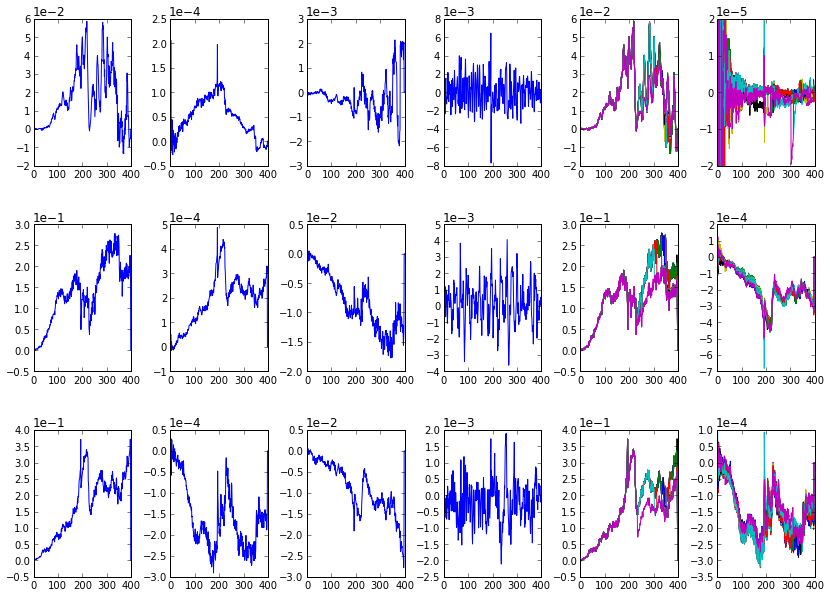
\includegraphics[width=12cm, keepaspectratio=true]
{./Figures/fltfig/cut1/Figure112.png}
\caption{State Vector Corrections}
\label{fltfig:4}
\end{figure}

\FloatBarrier

\section{Compare to Visually Corresponded Landmark}
\label{sec:flight-manual}
Due to the difficulty in corresponding landmarks extracted from video
to DEM, a second piece of video was processed with man-made structure
in the scene so that landmarks correspondence can be made manually.
Landmarks coordinates ground truth were taken from Google Earth. Since
Google Earth provided very rough elevation data, elevation of the
landmarks were taken from the GPS measurement of the helicopter when
it was landed at the airport. Figure \ref{fltfig:11} showed a
zoomed-in view of the landmarks extracted by the CC\_EKF\_SLAM. All
landmarks were located at the bottom left corner of the image. Figure
\ref{fltfig:12} showed the common landmarks found manually on the
satalite image on Google Earth \cite{_google_????}.

\begin{figure}[h]
\centering
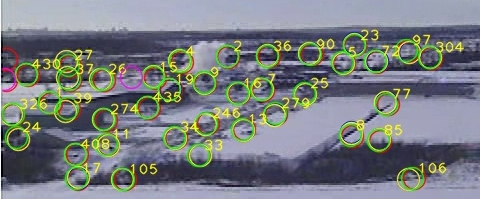
\includegraphics[width=10cm, keepaspectratio=true]
{./Figures/fltfig/airport/frame398_landmarks.jpg}
\caption{Landmark identified by algorithm }
\label{fltfig:11}
\end{figure}

\begin{figure}[h]
\centering
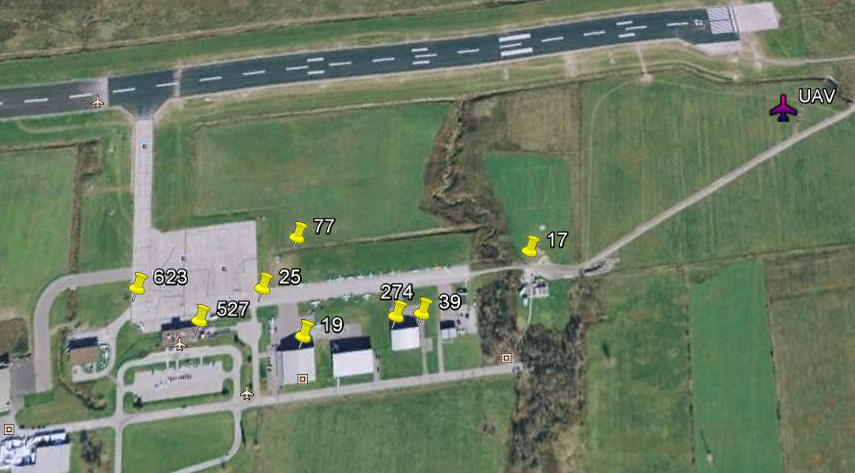
\includegraphics[width=13cm, keepaspectratio=true]
{./Figures/fltfig/airport/uav_and_identified_landmark.png}
\caption{Common landmarks identified manually on Google Earth }
\label{fltfig:12}
\end{figure}
\FloatBarrier The estimated SUAS poses were compared to onboard GPS
and IMU recordings in figure \ref{fltfig:13}. Similar to the natual
scene video, SUAS position estimates were more accurate on X and Z,
and experienced more drift on Y axis. The drift become significant
when frame number exceeds 200. The correlation between position error
and the rotational motion of the aircraft can also be found in this
plot.

\begin{figure}[h]
\centering
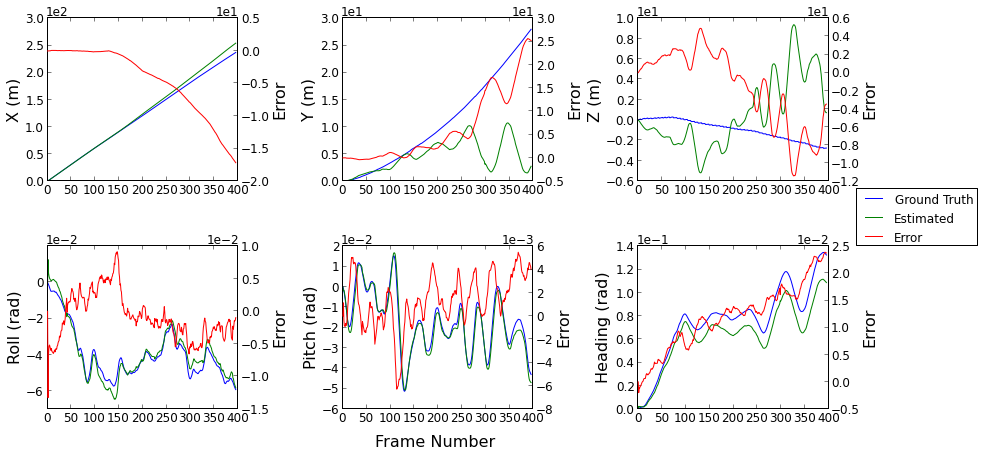
\includegraphics[width=17cm, keepaspectratio=true]
{./Figures/fltfig/airport/Figure10.png}
\caption{SUAS poses accuracy compared to ground truth}
\label{fltfig:13}
\end{figure}
\FloatBarrier

Figure \ref{fltfig:15} showed the landmarks positions compared to
ground truth. This plot showed a clear offset error between the ground
truth and the estimated. X axis coordinate had a mean offset of about
150 meters, and Y axis coordinate has a offset of about 60m. Since the
error existed on all landmark regardless of their ID value, and all
landmarks were located at the bottom left corner of the FOV, it is
likely that lens distortion was the main contributor to these error.


\begin{figure}[h]
\centering
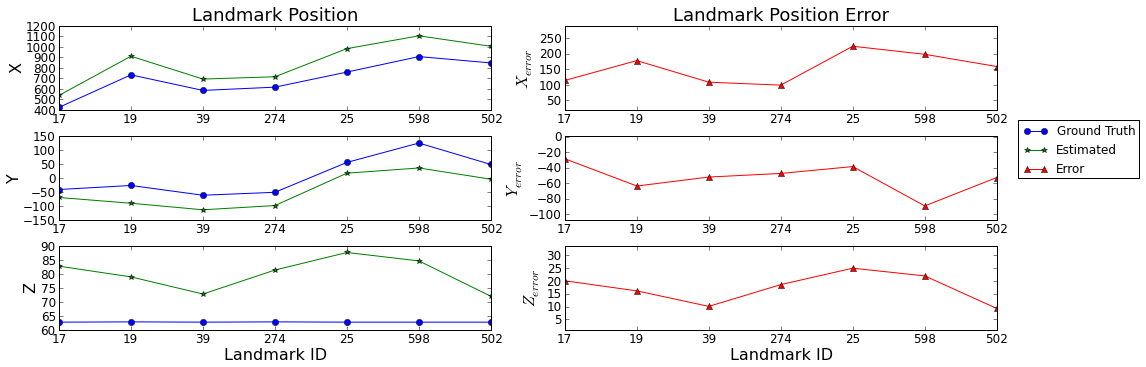
\includegraphics[width=17cm, keepaspectratio=true]
{./Figures/fltfig/airport/Figure20.png}
\caption{Landmarks positions compared to ground truth}
\label{fltfig:15}
\end{figure}

%%% Local Variables:
%%% mode: latex
%%% TeX-master: "thesis"
%%% End:
